\tikzstyle{decision} = [diamond, draw, fill=blue!20, 
    text width=4.5em, text badly centered, node distance=3cm, inner sep=0pt]
\tikzstyle{block} = [rectangle, draw, fill=blue!20, 
    text width=5em, text centered, rounded corners, minimum height=2em]
\tikzstyle{line} = [draw, -latex']
\tikzstyle{cloud} = [draw, ellipse,fill=red!20, node distance=3cm,
    minimum height=2em, text centered]
   
   
\newsavebox\myboxa
\savebox\myboxa{%
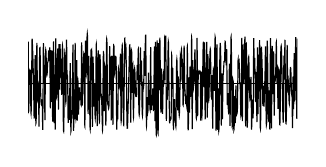
\begin{tikzpicture}[samples=500, domain=0:1*360]
        \begin{axis}[
            width=5cm, height=3cm,
            enlarge x limits=false,
            xtick=\empty,
            axis lines*=middle,
            hide y axis
        ]
        \addplot [no markers, smooth] {rand*2};
        \end{axis}
    \end{tikzpicture}%
}
    
% \tikzstyle{diamond} = [draw, diamond, node distance=3cm,
%     minimum height=2em]
    
\begin{tikzpicture}[node distance = 2cm, auto]
    % Place nodes
     \node [draw=none] (midiin) {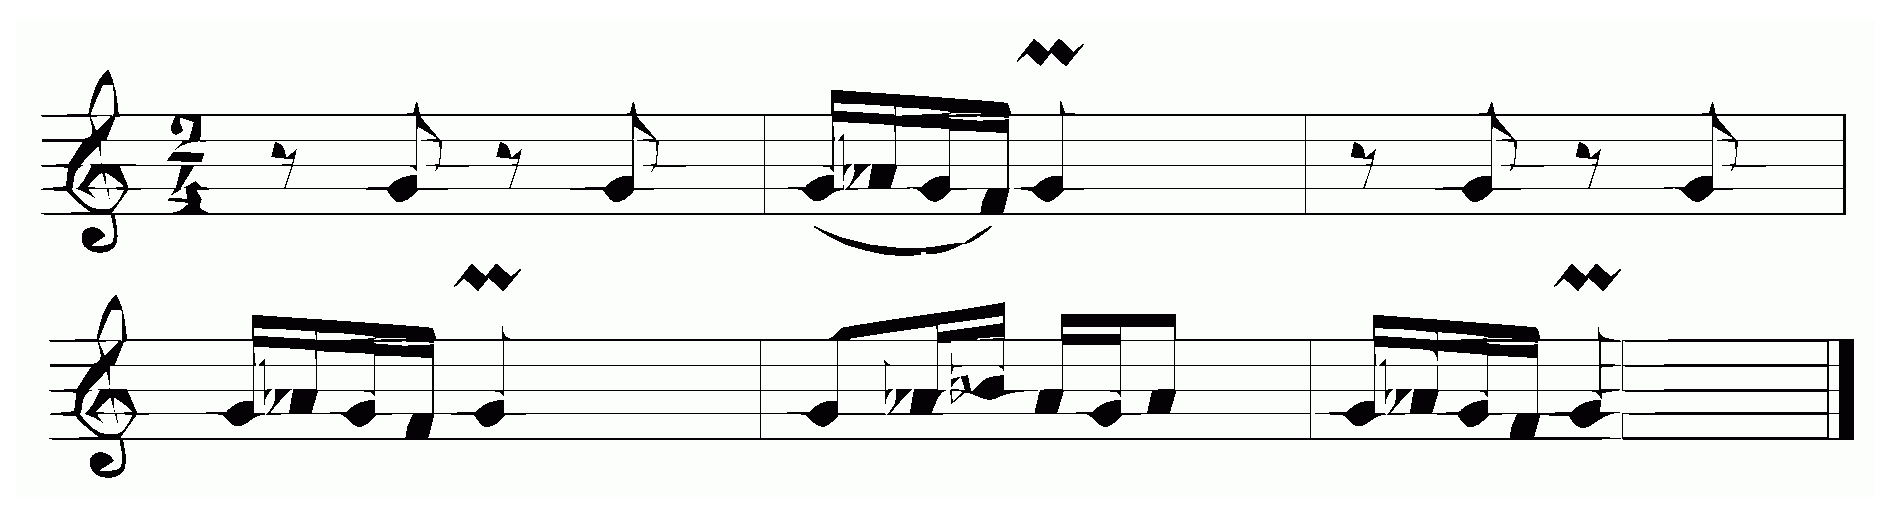
\includegraphics[width=.25\textwidth]{images/music/jambot/sheetmusic.eps}};
    \node [decision, below of = midiin, node distance = 2.5cm] (preprocessing) {pre processing};

%     \node [decision, left of = preprocessing] (midiin) {MIDI Input \eighthnote\eighthnote\eighthnote};

    \node [cloud, below left of = preprocessing] (chords) {chords};
    \node [cloud, below right of = preprocessing] (piano rolls) {piano rolls};
    \node [block, below of = preprocessing, node distance = 3cm] (chordlstm) {chord LSTM};
    \node [block, below of = chordlstm, xshift=-0.5cm] (melodylstm) {polyphonic LSTM};
    \node [cloud, right of = melodylstm, xshift=0.5cm, text width=5em] (predchords) {generated chord progression};
    
%     \node [decision, below of = melodylstm] (midiout) {MIDI Output \eighthnote\eighthnote\eighthnote};
         \node [draw=none, left of = melodylstm, node distance = 5cm] (midiout) {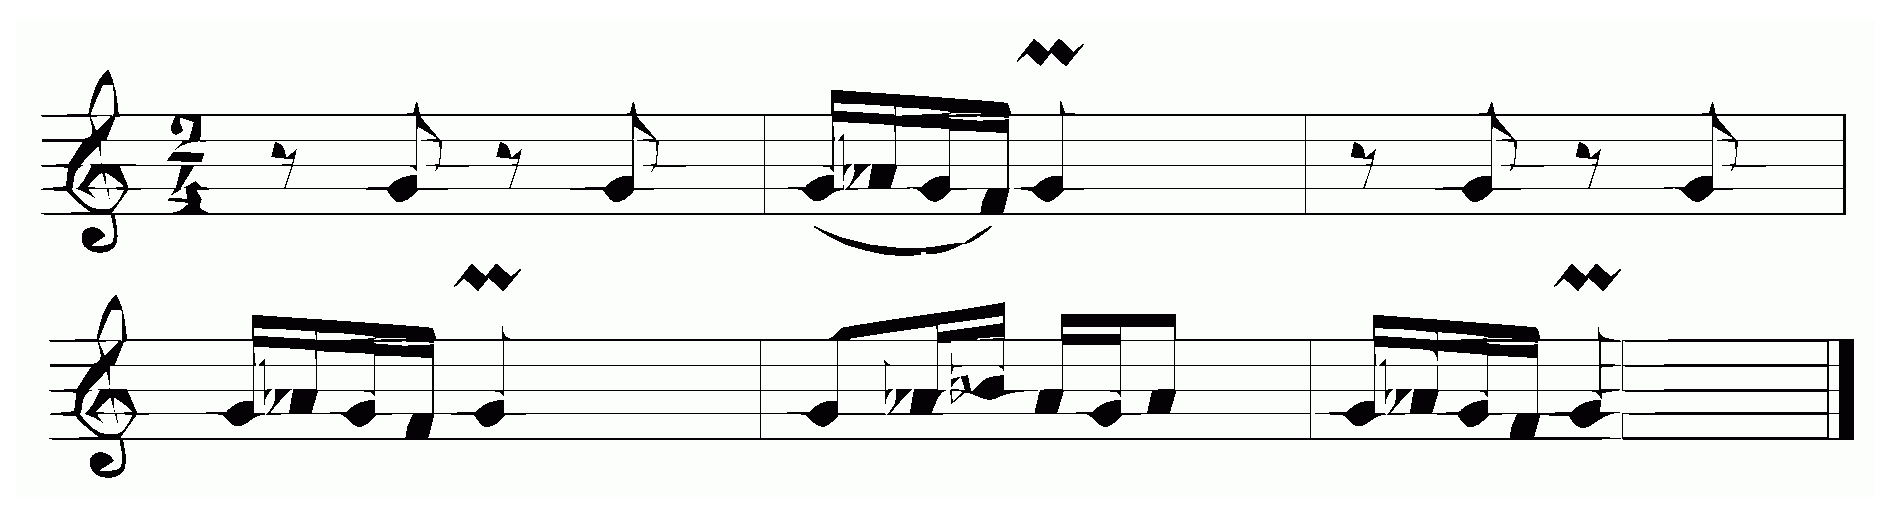
\includegraphics[width=.25\textwidth]{images/music/jambot/sheetmusic.eps}};
         
         %     \node [draw=none,below of = midiout, node distance =4cm] (musicout) {\usebox\myboxa};
    \node [draw=none,left of = midiout, node distance =4cm] (musicout) {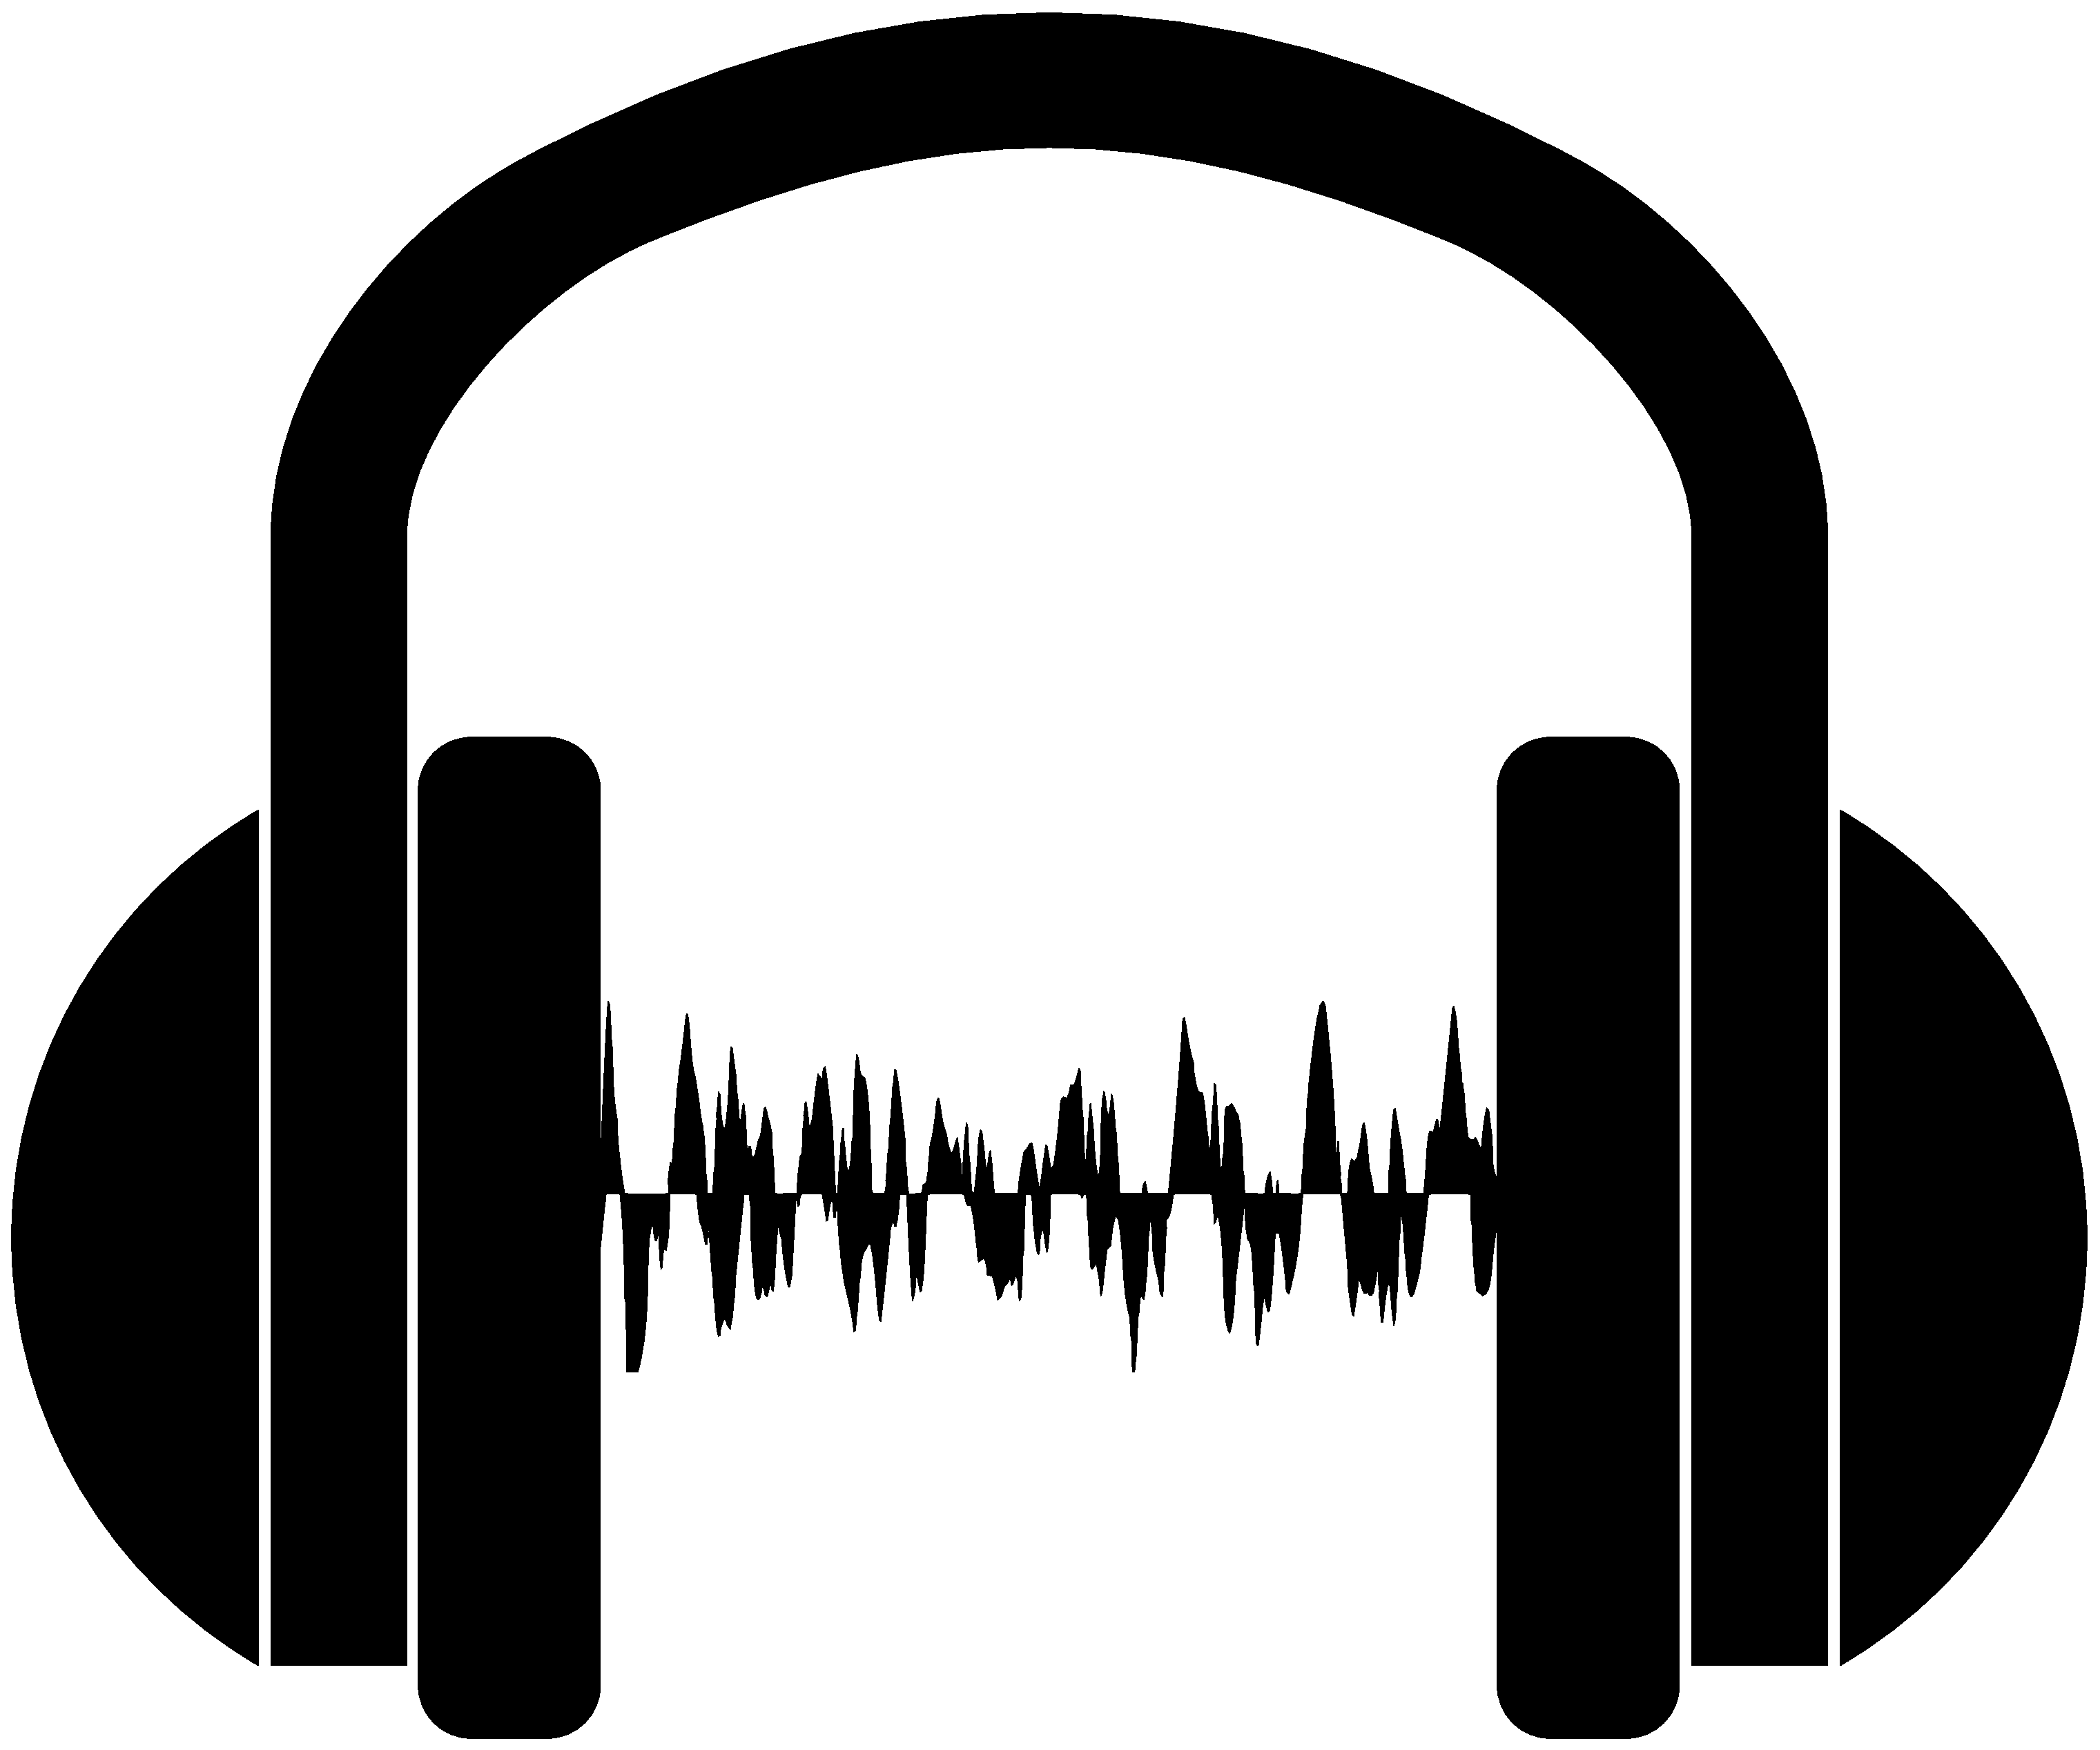
\includegraphics[width=.1\textwidth]{images/music/jambot/soundwaveheadphones.eps}};
         
     \node [cloud, above left of = musicout] (tempo) {tempo};
    \node [cloud, above right of = musicout] (instrumentation) {instrumentation};
    

    
    
    % Draw edges
     \path [line] (midiin) -- node[midway]{input MIDI training data}(preprocessing);
     \path [line, line width=0.5mm, black] (preprocessing) -- node [midway]{extract}(chords);
     \path [line, line width=0.5mm, black] (preprocessing) -- node [midway]{extract}(piano rolls);
     \path [line, line width=0.5mm, red] (chords) -- node [midway]{train}(chordlstm);
     \draw[bend right,->, line width=0.5mm, red] (chords) to node [midway, left]{train}(melodylstm);
      \draw[bend left,->, line width=0.5mm, red]  (piano rolls) to node [very near start]{train}(melodylstm);
      \path [line, line width=0.5mm, blue] (chordlstm) -- node [near end]{generate}(predchords);
      \path [line, line width=0.5mm, blue] (predchords) -- node [midway]{input}(melodylstm);
      \path [line, line width=0.5mm, blue] (melodylstm) -- node [midway]{generate MIDI}(midiout);
      \path [line, line width=0.5mm, blue] (midiout) -- (musicout);
      \path [line, line width=0.5mm, blue] (tempo) -- (musicout);
      \path [line, line width=0.5mm, blue] (instrumentation) -- (musicout);
%     \path [line] (decide) -| node [near start] {yes} (update);
%     \path [line] (update) |- (identify);
%     \path [line] (decide) -- node {no}(stop);
%     \path [line,dashed] (expert) -- (preprocessing);
%     \path [line,dashed] (system) -- (preprocessing);
%     \path [line,dashed] (system) |- (evaluate);
\end{tikzpicture}
